\chapter{Language Usage Tutorial}

This will cover the configuration of the user's environment and the usage of Extend's features.

\section{Setup}
The Extend compiler requires that the OCaml Language and LLVM be installed on the host machine. Development was done in a virtual machine running the 64-bit Ubuntu operating system. In order to quickly get Extend up and running, please use \underline{\href{https://courseworks2.columbia.edu/courses/10787/files/673708/download}{this virtual machine}}, which has been provided as part of the course.

	\medskip \noindent After booting up the virtual machine, clone the Extend git repository:

	\begin{lstlisting}
		git clone https://github.com/ExtendLang/Extend.git
	\end{lstlisting}

\section{Compiling and Running Extend Code}
To build the Extend compiler, the first steps are the following.

	\begin{lstlisting}
cd Extend/
make
	\end{lstlisting}

	\medskip \noindent
	If this does not successfully build, run \texttt{eval `opam config env`}, which should configure the environment to use OPAM packages. Alternatively, add this command to your bash profile.

	 \medskip \noindent
	 After running \texttt{make}, you should see a \texttt{main.byte} file. To compile and run an Extend program, we have provided a shell script to simplify the process for the user:

	\begin{lstlisting}
	./compile.sh example_source_file.xtnd
	\end{lstlisting}

	\medskip \noindent
	This should produce an \texttt{out} file. Running \texttt{./out} should successfully execute the program.
\section{Illustrating the Benefits of Extend}
Spreadsheet applications require the use of manual input in order to apply the same calculation to a different set of data. Extend aims to tackle this problem by offering portability. Below is an example of a spreadsheet user calculating the unit vector of a column vector:

\begin{center}
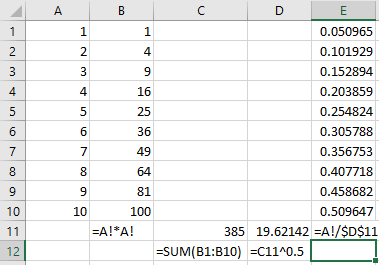
\includegraphics[width=7cm]{img/unitvector.png}
\end{center}

\medskip \noindent The Excel user must manually input the data, and additionally make space for the intermediate steps of the calculation. As the data becomes more diverse and the problem becomes more complicated, more work is required. Below is the equivalent function in Extend, written to work on any column vector that is passed in:

\begin{lstlisting}
	normalize_column_vector([m,1] arg) {
	  [m,1] squared_lengths := #arg * #arg, normalized := #arg / vector_norm;
	  vector_norm := sqrt(sum(squared_lengths));
	  return normalized;
	}
\end{lstlisting}

\medskip \noindent Another particularly interesting example is concatenating a row of strings of variable length with a common delimiter. This in an entirely manual operation for the spreadsheet user; a step-by-step attempt is shown below.

\begin{center}
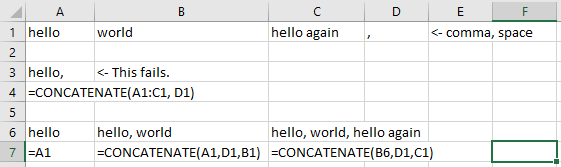
\includegraphics[width=9cm,height=3cm]{img/concatenation.png}
\end{center}

\medskip \noindent Performing a delimiter 'join' like the above can be performed in a simple program in Extend without knowing the size of the row.

\begin{lstlisting}
main(args){
	bar := {"Hello", "Goodbye", "Hello Again"};
	str := ", ";
	return foo(bar, str);\\ prints "Hello, Goodbye, Hello Again"
}

foo([1,n] colrange, str){
	[1,n] baz;
	baz[0,0] = #colrange;
	baz[0,1:] = baz[0,[-1]] + str + colrange[0,[0]];
	return print_endline(baz[0,-1]);
}
\end{lstlisting}

\medskip \noindent As evidenced above by simple examples, Extend offers flexibility that is significantly harder to achieve with conventional spreadsheet applications. As the nature of the data grows in complexity and variety, Extend's value increases.

\section{Writing Extend Code - The Basics}
Extend code can be written in a file that contains the conventional \texttt{.xtnd} extension. It consists of optional import statements and global variables, and an optional set of functions. Runnable Extend programs must contain a \texttt{main} function, and other functions can be written into the program as well.

\medskip \noindent
Below is a short tour of the features of Extend. More detail can be found in the next chapter - the Language Reference Manual.

	\subsection{Functions}
	Functions are commonplace in Extend. They are declared with the syntax \texttt{function\_name([optional\_dimensions] function\_arguments)\{...\}}. Below is the syntax of the \texttt{main} function, which is needed to run Extend code, within a simple Extend program.

	\begin{lstlisting}
	main(args){
			return 0;
	}
	\end{lstlisting}
	% Perhaps a more informative program - but not too difficult.

	\medskip \noindent
 	The return type of a function is a value that can be of any type or dimensions. \textbf{Ranges} will be discussed in a later section of this chapter. A function is composed of variable declarations and formula assignments and concludes with the \textbf{return} statement.
	Note that the \textbf{return} statement is always the last statement in the function.

		\subsubsection{Function Parameters}
		Function parameters consist of zero or more ranges, signed with an optional dimension. If the arguments have been written with dimensions, those dimensions will be verified at runtime.
		\begin{lstlisting}
			foo([m,n] arg){
				return m * n; \\ m and n initialized through arg1
			}

			bar([1,1] arg){
				return 0; \\ 1 by 1 ranges should be primitive data types. If arg is not, a runtime error will be thrown
			}
		\end{lstlisting}

	\subsection{Adjusting to Extend's Declarative Nature}
	The biggest difference between Extend and most traditional programming languages is that the concept of an imperative statement does not exist. An Extend function consists solely of variable declarations, formula assignments, and a return expression. When a function is called, its \texttt{return} expression is evaluated, along with the values of any variables that the return expression depends on. In a traditional imperative language, the order of operations is determined explicitly by the developer; in Extend, the order is determined implicitly by the desired result.

	\medskip \noindent The following file compiles and prints successfully.

	\begin{lstlisting}
		main(args){
			foo := "Hello World!";     // Combined var declaration and formula assignment
			return print_endline(foo); // Return expression is a call to print_endline().
		}
	\end{lstlisting}

	\medskip \noindent However, the file below is not a legal Extend program:

	\begin{lstlisting}
		main(args){
			foo := "Hello World!"; // OK
			print_endline(foo);    // Not OK
			return foo;
		}
	\end{lstlisting}

	\medskip \noindent As illustrated, Extend only evaluates what is needed to produce the value required by \texttt{return}. Any non-essential declarations or formula assignments will be ignored by the program. If the user attempts to write statements like \texttt{print\_endline("Hello")} by itself, the program will not compile.

	\subsection{Data Types}
	Extend has three primitive data types: Numbers, Strings, and \texttt{empty}; and one composite type, Range. An example of each is shown below.

	\begin{lstlisting}
		myNumber    := 5;
		myString    := "Hello World";
		myEmpty     := empty;
		my2x3Range  := {3, 4, "five"; "a", "b", "c"};
	\end{lstlisting}

	\subsection{Variables}
	In Extend, \texttt{variables} are composed of cells to which formulas are assigned. The first time (and only the first time!) an individual cell is referenced by an expression, its value is calculated according to its assigned formula. A cell's value is not calculated if the cell is never referred to, and is never recalculated; all cell values are immutable. A cell's value can be any of Extend's types, and different cells of a single variable can have different types.

	\begin{lstlisting}
		[1,2] foo; // Declares a variable with 1 row and 2 columns (2 cells total)
		[1,3] bar := 4; // Declares a variable with 1 row and 3 columns and
		                // assigns the literal value 4 as the formula for each cell
		[1,2] baz;                 // Declares a 1x2 variable baz
		baz[0,0] = "first";   		 // Assigns literal "first" as the formula for the
		baz[0,1] = 1 + 1;          // 1st cell and the expression 1+1 for the 2nd cell
		life := 6, universe := 7;  // Declares 1x1 variables life and universe
		answer := life * universe; // Declares a 1x1 variable the_answer and assigns
															 // the formula life * universe to its sole cell
		[1,10] half_and_half;			 // Declares a 1x10 variable half_and_half
		half_and_half[0,0:5] = "milk";		// Assigns "milk" to the first five cells
		half_and_half[0,5:10] = "cream";  // and "cream" to the second five cells
	\end{lstlisting}

	\medskip \noindent
	\textbf{Note} that we declare a variable and assign a formula to all of its cells in a single line with \texttt{:=}. If the variable has already been declared, a formula must be assigned using \texttt{=} instead of \texttt{:=}. As illustrated in this example, a single formula can be assigned to multiple cells of a variable with the slice syntax. The converse is not true: multiple formulas applying to a single cell will cause a runtime error. The contents of the slice, as well as the dimensions of the variable, can be any expression that evaluates to a number, not just a literal number. For example, this code snippet assigns the dimensions based on the \texttt{howBig()} function and the "left" and "right" formulas based on the \texttt{breakpoint()} function:

	\begin{lstlisting}
		breakpoint() {
			return 7;
		}
		howBig() {
			return 11;
		}
		foo_func() {
			[1,howBig()] foo;
			foo[0, :breakpoint()] = "left";
			foo[0, breakpoint():-1] = "right";
			foo[0, -1] = "last";
			return foo;
		}
	\end{lstlisting}

	\medskip \noindent
	This example also illustrates that the start (or end) index of a slice can be omitted if the developer wants the formula to apply from the beginning (or to the end) of the dimension, and that negative numbers can be used in a slice to count backwards from the end. As with all values in Extend, the dimensions of a variable, and the slices to which a formula applies, are immutable. The first time a variable is referred to (directly or indirectly) by the return expression, its dimensions and the formula assignment slices are computed; from that point on, they never change. In the example above, the howBig() function is invoked once, but the breakpoint() function is actually called twice: once for the "left" formula, and once for the "right" formula.

	\subsubsection{Variables vs. Ranges}
	A variable is not a data type; it is a collection of one or more cells with assigned formulas. A range is a value, which is internally implemented as a pointer to a subset of a variable's cells. A range is always composed of more than one value; a variable may have a single cell. The variable "backing" a range may not have been explicitly defined by the developer; for example, range literals are implemented using an anonymous variable.

	\subsection{Operators}
	Extend includes a comprehensive set of operators. Each category is listed in order of precedence. A more detailed explanation of each operator can be found in the Language Reference Manual.

		\subsubsection{Arithmetic Operators}
			\begin{itemize}
				\item Unary Operations: \texttt{-}
				\item Binary Operations: \texttt{**, *, /, \%, +, -}
			\end{itemize}

		\subsubsection{Bitwise Operators}
			\begin{itemize}
				\item Unary Operations: \texttt{\~}
				\item Binary Operations: \texttt{<<, >>, \&, |, \^}
			\end{itemize}

		\subsubsection{Boolean Operators}
			\begin{itemize}
				\item Unary Operations: \texttt{!}
				\item Binary Operations: \texttt{==, !=, <, >, <=, >=, \&\&, ||}
			\end{itemize}

		\subsubsection{String Concatenation}
		Note that the \texttt{+} symbol can be used to perform concatenation between two strings.

		\begin{lstlisting}
			"Hello " + "World\n"
		\end{lstlisting}

		\subsubsection{The size and typeof operators}
		Extend offers a \texttt{typeof(expr)} operator, which takes an expression and returns Number, String, Range, or Empty (as a string). It also has the \texttt{size(expr)} operator, which returns the dimensions of its argument as a 1 x 2 range.


	\subsection{Conditionals}
	There are two types of conditional expressions: the if-then-else (ternary) conditional and a \texttt{switch} expression.

		\subsubsection{If-Then-Else}
		The two equivalent ways to write the ternary expression are as follows: \newline \newline
		C/Java style: \texttt{condition ? expr\_if\_true : expr\_if\_false} \newline \newline
		Spreadsheet style: \texttt{if(conditional, expr\_if\_true, expr\_if\_false)}

		\subsubsection{The Switch Expression}
		Below is an example of the switch expression used in a function:

		\begin{lstlisting}
			odd_or_even(foo){
				return switch(foo % 2) {
					case 0: "Even";
					case 1: "Odd";
					default: "Not an integer";
				};
			}
		\end{lstlisting}

	\medskip \noindent
	In the example above, the \texttt{switch} expression used foo % 2 as an argument; however, this is not required, so a switch expression can be used (as in Go) as a replacement for a sequence of if-then-else conditionals.

		\subsubsection{Range Slicing \& Selection}
		Python-style array-slicing syntax can be applied to ranges, which will return a subrange based on either absolute or relative indexing. All indices are zero-based.

		\begin{lstlisting}
			foo[0,2] \\ The cell in the first row, third column
			foo[0,:] \\ The range of cells in the first row
			foo[0,[1]] \\ The range in the column that is 1 column right of the left-hand-side cell.
			foo[,] \\ Cell in first row, first column if 1 by 1. If not, then relative first row and relative first column
		\end{lstlisting}

		\medskip \noindent
		More examples and detail can be found in the next chapter.

		\subsubsection{The Hash Operator}
		A common case for ranges in Excel is to perform calculations on specific cells. For example, \texttt{foo[,]} is commonly used to retrieve the cell that is being calculated on.
		Since this is a popular use case, the \texttt{\#} operator will perform the same functionality.

		\subsubsection{Application on Ranges}
		Extend, in the vein of spreadsheets, allows the programmer to apply functions cell-wise on a range. Using the \texttt{\#} operator, we can perform cell-wise multiplication across two ranges.

		\begin{lstlisting}
			foo([m,n] arg1, [m.n] arg2){
				[m,n] bar := #arg1 * #arg2; \\ Multiplies the cell in arg1 with the corresponding cell in arg2.
				return bar;
			}
		\end{lstlisting}

		\medskip \noindent
		This is an incredibly powerful aspect of Extend. Make sure to study it well!

		\subsubsection{Range Attribute Functions}
		Extend has the \texttt{row()} and \texttt{column()} functions, which respectively return the row and column of the cell that is being calculated at that point in time.
		There is also a \texttt{size(expr)} function, which returns a 1 by 2 range; the first cell contains the number of rows, and the second cell contains the number of columns.

	\subsection{Cell Evaluation, Side Effects, and Precedence Expressions}
	As mentioned before, a cell's value is calculated at most once. It is evaluated when it is the only cell selected from a variable, or when a selection containing the cell is assigned as a range to another cell. In general, the language is designed so you don't have to think about this! However, in the case of formulas that call functions with side effects, it's important to understand the behavior. When necessary, a precedence expression (using the \texttt{->} operator) can be used to force the evaluation of one expression before another. A precedence expression calculates the first expression, discards the result, and evaluates to the second expression. The following example should help clarify how cell evaluation is performed:

	\begin{lstlisting}
	main(args) {
		foo := print_endline("Once") -> 2;
		bar := foo + foo;
		return print_endline(bar);
	}
	\end{lstlisting}

	\medskip \noindent
	This program prints "Once" and then prints 4. Before calling print\_endline, Extend calculates the value of bar, which in turn requires the value of foo (twice). The first time foo's value is calculated, print\_endline() is called with the argument "Once", and then foo evaluates to the constant 2. The second time that foo's value is required to calculate bar, it's already available: it is 2. Therefore, print\_endline("Once") is not called a second time.

	\subsection{Import Statements}
	In Extend, you can import other Extend files at the top of your program via relative directory path. The use case is below:

	\begin{lstlisting}
		import "../programs/helloworld.xtnd"
	\end{lstlisting}

\section{Standard Library Functions}
Extend offers an assortment of standard library functions. Extend imports \texttt{stdlib.xtnd}, which has aggregated all the standard library functions for the user's disposal.

\medskip \noindent
While their usage will be covered in more length in the Language Reference Manual, here are some of the more useful standard library functions to remember.
	\subsection{Basic Functions}
		\subsubsection{The toString() Function}
		The \texttt{toString()} function takes a 1 by 1 range and renders its value as a string. This will return one of the primitive data types.

		\begin{lstlisting}
			return "Hello " + toString(14); \\ "Hello 14"
		\end{lstlisting}

		\subsubsection{Math Functions}
		Borrowing from C's standard library math functions, Extend offers: \texttt{sin, cos, tan, acos, asin, atan, sinh, cosh, tanh, exp, log, log10, sqrt, ceil, fabs} and \texttt{floor}.

		\begin{lstlisting}
			main(args){
				bar := sqrt(16);
				return write(STDOUT, toString(bar)) -> 0; \\ Prints 4 to stdout
			}
		\end{lstlisting}

	\subsection{File I/O}
	Extend has \texttt{open, close, read, and write} functions to interact with files. Usage is as follows:

	\begin{lstlisting}
		main(args){
		  return write(STDOUT, read(open("test_file.txt", "r"),5)) -> 0; \\ Writes 5 characters from test_file.txt to stdout
		}
	\end{lstlisting}

	\subsection{Plotting}
	Extend also offers the ability to export plots to a PNG file with the \texttt{plot} function.

	\begin{lstlisting}
		TODO: Demonstrate usage here.
	\end{lstlisting}
